% Author: Rasmus Pank Roulund
\documentclass{standalone}
\usepackage{tikz}
\usetikzlibrary{shapes.geometric, arrows, positioning, calc, fit, arrows, decorations.pathreplacing}

\newcommand\drawcontrol[3]{%
    \draw[control] ($(#1*\xd,#2*\xd)+(xc)$) -- ++(#3);
}

\begin{document}

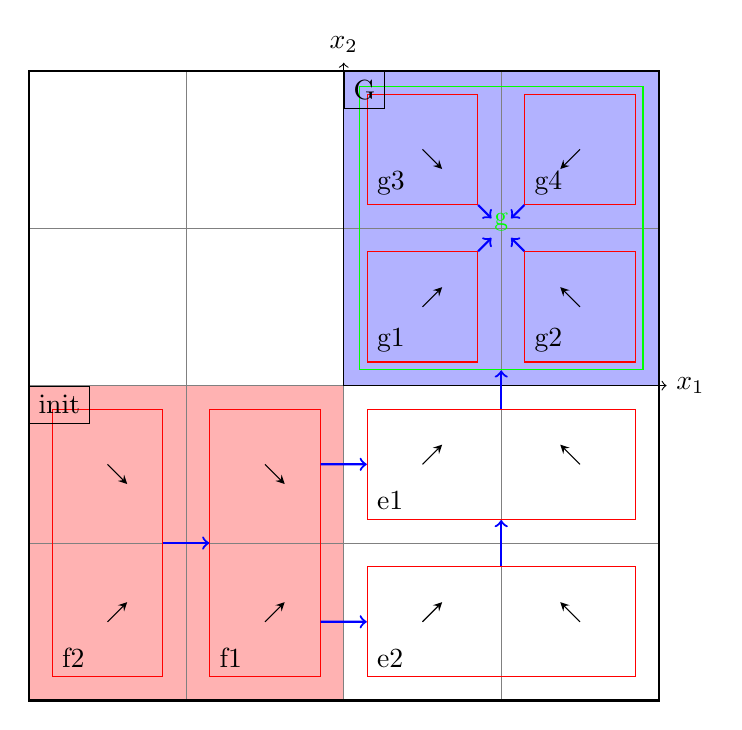
\begin{tikzpicture}[]
    
\tikzstyle{control}  = [->,>=stealth]
\tikzstyle{controlrect}  = [red]
\tikzstyle{transition}  = [->,blue,thick]
\tikzstyle{myrect}  = [
  rectangle,
  draw,
  inner sep=0pt,
  fit=#1,
  red]
    
\def\outsize{1.25}
\draw[draw=none] (-\outsize,-\outsize) rectangle (\outsize,\outsize); 

\def\xm{4.}
\def\xd{2}
\def\u{0.5}

\draw[fill=blue!30!white] (0,0) rectangle (\xm,\xm);
\draw[fill=red!30!white] (-\xm,-\xm) rectangle (0.,0.);

\draw[step=\xd cm,gray,very thin] (-\xm,-\xm) grid (\xm,\xm);
\draw[thick] (-\xm,-\xm) rectangle (\xm,\xm);

\draw[<->] (0,\xm+0.1) node (yaxis) [above] {$x_2$}
        |- (\xm+0.1,0) node (xaxis) [right] {$x_1$};


\coordinate (xc) at (\xd/2,\xd/2);
\coordinate (xr) at (\xd/2-0.3,\xd/2-0.3);
\coordinate (xg) at (\xd/2-0.2,\xd/2-0.2);

\coordinate (unw) at (-\u/2,\u/2);
\coordinate (une) at (\u/2,\u/2);
\coordinate (usw) at (-\u/2,-\u/2);
\coordinate (use) at (\u/2,-\u/2);

\def\cont#1#2#3{\draw[control] ($(#1*\xd,#2*\xd)+(xc)$) -- ++(#3)}

\def\rect#1#2#3#4#5{
\coordinate (xa) at ($(#1*\xd,#2*\xd)+(xc)-(xr)$);
\coordinate (xb) at ($(#3*\xd,#4*\xd)+(xc)+(xr)$);
\node(#5)[myrect={(xa) (xb)}] {};
\node[anchor=south west] at (xa) {#5};
}

\def\goal#1#2#3#4#5{
\coordinate (xa) at ($(#1*\xd,#2*\xd)+(xc)-(xg)$);
\coordinate (xb) at ($(#3*\xd,#4*\xd)+(xc)+(xg)$);
\node(#5)[myrect={(xa) (xb)},green] {#5};
}

\cont{-2}{-2}{une};
\cont{-2}{-1}{use};
\cont{-1}{-2}{une};
\cont{-1}{-1}{use};

\cont{0}{-2}{une};
\cont{1}{-2}{unw};
\cont{0}{-1}{une};
\cont{1}{-1}{unw};

\cont{0}{0}{une};
\cont{1}{0}{unw};
\cont{0}{1}{use};
\cont{1}{1}{usw};

\rect{0}{0}{0}{0}{g1};
\rect{1}{0}{1}{0}{g2};
\rect{0}{1}{0}{1}{g3};
\rect{1}{1}{1}{1}{g4};

\rect{0}{-1}{1}{-1}{e1};
\rect{0}{-2}{1}{-2}{e2};

\rect{-1}{-2}{-1}{-1}{f1};
\rect{-2}{-2}{-2}{-1}{f2};

\goal{0}{0}{1}{1}{g};

\draw[transition] (f2.east) -- (f1.west);

\coordinate (a1) at (intersection of e2.west--e2.east and f1.north east--f1.south east);
\coordinate (a2) at (intersection of e1.west--e1.east and f1.north east--f1.south east);
\draw[transition] (a2) -- (e1.west);
\draw[transition] (a1) -- (e2.west);
\draw[transition] (e2.north) -- (e1.south);

\draw[transition] (e1.north) -- (g.south);

\draw[transition,shorten >=5pt] (g1.north east) -- (g.center);
\draw[transition,shorten >=5pt] (g2.north west) -- (g.center);
\draw[transition,shorten >=5pt] (g3.south east) -- (g.center);
\draw[transition,shorten >=5pt] (g4.south west) -- (g.center);

\node[draw,anchor=north west] at (0,\xm) {G};
\node[draw,anchor=north west] at (-\xm,0) {init};

\end{tikzpicture}

\end{document}
